\cleardoublepage
\chapter{Diskusjon}
\label{chap:discussion} 

I dette kapittelet vil resultatet bli diskutert. Kapittelet vil fokusere på om resultatet ble som forventet, om oppdragsgiver var fornøyd med resultatet, om gruppen gjort noe annerledes/bedre og hva gruppen har lært underveis. Det vil også inneholde en vurdering av produktet opp mot relatert arbeid. Gruppen vil gi anbefalinger og fremlegge designprinsipper for videre arbeid og utvikling av plattformen i praksis. Til slutt er en konklusjon med oppsummering av arbeidet og prosessen.

\section{Resultat i forhold til oppdragsgivers forventinger}

\section{Resultat i forhold til sluttbrukerens krav}

\section{Gruppens evaluering}

\section{Vurdering av produkt opp mot relatert arbeid}

\section{Erfaringer gjort underveis}
\subsection{Hva kunne blitt gjort annerledes?}

\section{Anbefalinger for utvikling og videre arbeid}
\subsection{Database}
Siden systemet inkluderer innlogging og informasjon fra andre kilder enn Brønnøysundregisteret er det behov for en database som lagrer passord, brukernavn og øvrig info om både brukere, organisasjoner og administrator. Figur~\ref{fig:databasemodell} viser en modell av informasjonen som lagres i databasen.

Koblingene mellom tabellene viser til at hver organisasjon kan ha flere brukerprofiler tilknyttet seg, samtidig som hver bruker kan være tilknyttet flere organisasjoner. Hver bruker kan også være tilknyttet flere andre brukere.

Inkludert i systemet er et administratorpanel der så mye som mulig er automatisert i systemet, slik at det ikke trengs mer enn 5-10 minutter per uke med vedlikehold fra administrator sin side.
\\
\begin{figure}[H]
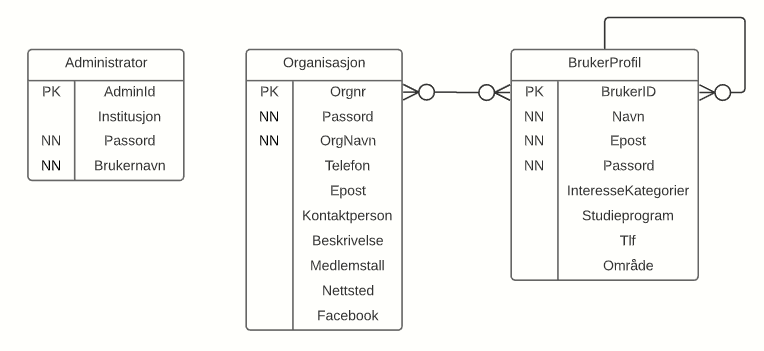
\includegraphics[width=\textwidth]{Illustrasjoner/databasemodell-2.png}
\caption{Databasemodell for lagring av informasjon for Administrator, Organisasjon og Brukerprofil}
\label{fig:databasemodell}
\end{figure}

\subsection{Feide og tilgang til studentinformasjon}

\subsection{Merkevarebygging og synliggjøring av produktet}

Produktet blir laget i samkoordinering med Høgskolen i Østfold som et av deres bachelorprosjekter. Dette alene gir stor vekt blant aktører og organisasjoner som vil kunne være interessert i et slikt produkt, enda mer om Høgskolen i Østfold offentlig stiller seg bak produktet og bruker det som en del av sin hjemmeside.

Utfordringen blir å skape et levende produkt, hvor organisasjoner legger inn egen informasjon og sørger for at ny og oppdatert informasjon blir lagt til kontinuerlig. Dette innebærer at det må være attraktivt for organisasjoner og legge til informasjon og oppdatere sine sider inne på plattformen.

\paragraph{Hvordan kan dette løses?}

Produktet må være godt synlig og lett tilgjengelig plassert på fremsiden til Høgskolen i Østfold for at dette produktet skal bli brukt av studenter. det anbefalles også at det blir kjørt et redesign av HIØ sitt nettsted ettersom det er ganske kaotisk på nåværende tidspunkt. For at det skal være attraktivt for organisasjoner å legge inn og oppdatere sin informasjon så skal det introduseres ett system som plasserer organisasjoner med oppdatert informasjon lengre opp på resultat listene. I tillegg skal det i start fasen av produktet kontaktes en del store organisasjoner for å få de til å legge til informasjon om seg selv som igjen kan starte et initiativ hos andre til å legge til sin informasjon. 


\paragraph{Markedsføring opp mot studenter}

Dette produktet er laget for nye studenter ved høgskolen og skal hjelpe dem i starten av studie tiden for å finne fritids aktiviteter og organisasjoner å ta del i. Resultater i være brukertester og undersøkelser viser at dette er noe nåværende studenter ønsker fantes da de startet, og noe kommende studenter sier hadde vært et bra tiltak for dem når de skal studere. 
undersøkelsene våre viser at dette produktet er noe som må introduseres så tidlig som mulig i studietiden. gruppens hovedtips til utviklere og administrator er at dette produktet må ha en sentral rolle på høgskolens nettside, introduseres i fadderukene og markedsføres gjennom student politikken og student organisasjoner.

\paragraph{Markedsføring opp mot organisasjoner}

Markedsføringen opp mot organisasjoner i starten er en god del manuell jobb for administrator for dette produktet hvor administrator selv må sende ut invitasjoner og rekrutere organisasjoner til siden. Derfor er det viktig for utviklere og automatisere så mye av prosessen når det kommer til rekruttering som mulig. Men all jobben som legges ned i oppstarten av dette produktet vil være vel verdt det etterhvert når produktet blir mer kjent blant organisasjoner å de selv kommer til siden for å registrere seg. Etterhvert når merkevaren blir godt kjent og kanskje har spred seg ved å bli tilbudt eller tatt opp av andre instanser, håper vi at dette vil skape en type bevegelse blant organisasjoner i Norge hvor det å være en del av merkevaren "Aktiv Student" er attraktivt og hjelper til å berike organisasjons samfunnene og nærområdene rundt. Gruppens hovedtips for utviklere og administrator er å starte med studentorganisasjonene å få med alle disse så det vises at høgskolen stiller seg bak. Noe som kan hjelpe merkevarebyggningen kraftig er å presentere dette produktet for de forskjellige organisasjons forbundene i Norge å få dem ombord, så de videre kan markedsføre dette videre til sine organisasjoner. Prøv å skape media dekking rundt merkevaren for å introdusere dette til nærmiljøet. 

\paragraph{Videre markedsføring og fremtidsplan for produktet}

Dette produktet blir bygget i hovedsak for HIØ. Men det betyr ikke at produktet kun begrenses til kommunene Fredrikstad, Sarpsborg og Halden. Informasjonen som hentes ut fra brreg.no dekker hele Norge. Det betyr at systemet har tilgang på all den informasjonen og ved noen enkle endringer på område parameterene i programmet til produktet kan det tilbys til for eksempel andre høyskoler, kommuner, fylker og interesserte parter. Det vil si at produktet kan da tilbys til andre nettsteder, som vil skape et større navn for vår merkevare. dette er med på å få de forskjellige organisasjonene til å se på det som attraktivt å legge inn sin informasjon som vil skape en god sirkel av merkevarebygging for alle parter.


\section{Konklusjon og oppsummering}







